\documentclass[12pt]{article}
\usepackage[english]{babel}
\usepackage[utf8x]{inputenc}
\usepackage{amsmath}
\usepackage{graphicx}
\usepackage{subcaption}
\usepackage[export]{adjustbox}
\graphicspath{ {./images/} }
\PassOptionsToPackage{hyphens}{url}
\usepackage{hyperref}

\usepackage{xcolor}

\definecolor{codegreen}{rgb}{0,0.6,0}
\definecolor{codegray}{rgb}{0.5,0.5,0.5}
\definecolor{codepurple}{rgb}{0.58,0,0.82}
\definecolor{backcolour}{rgb}{0.95,0.95,0.92}

\hypersetup{
    colorlinks=true,
    linkcolor=blue,
    filecolor=magenta,      
    urlcolor=blue,
}
\usepackage{listings}
\lstdefinestyle{mystyle}{
    backgroundcolor=\color{backcolour},   
    commentstyle=\color{codegreen},
    keywordstyle=\color{magenta},
    numberstyle=\tiny\color{codegray},
    stringstyle=\color{codepurple},
    basicstyle=\ttfamily\footnotesize,
    breakatwhitespace=false,         
    breaklines=true,                 
    captionpos=b,                    
    keepspaces=true,                 
    numbers=left,                    
    numbersep=5pt,                  
    showspaces=false,                
    showstringspaces=false,
    showtabs=false,                  
    tabsize=2
}
\lstset{style=mystyle}
 
\usepackage[colorinlistoftodos]{todonotes}

\begin{document}

\begin{titlepage}

\newcommand{\HRule}{\rule{\linewidth}{0.5mm}} 

\center
-------------------------------------------------------------------------------------

\textsc{\LARGE Politenico di Milano}\\[1cm]
\textsc{\Large Dipartimento Elettronica, Informazione e Bioingegneria}\\[0.5cm] 
\textsc{\large Embedded Systems Project}\\[0.5cm] 

%----------------------------------------------------------------------------------------
%	TITLE SECTION
%----------------------------------------------------------------------------------------

\HRule \\[0.4cm]
{ \huge \bfseries Square Root for bfloat16}\\[0.4cm]
\HRule \\[1.5cm]
 
%----------------------------------------------------------------------------------------
%	AUTHOR SECTION
%----------------------------------------------------------------------------------------

\begin{minipage}{0.4\textwidth}
	\begin{flushleft} \large
		\emph{Authors:}\\
		Francesco \textsc{Monti} \\
		Fabio \textsc{Nappi} \\
		Davide \textsc{Piovani} 
	\end{flushleft}
\end{minipage}
~
\begin{minipage}{0.4\textwidth}
	\begin{flushright} \large
		\emph{Supervisor:} \\
		Dr. Davide \textsc{Zoni}
		Dr. Andrea \textsc{Galimberti}
	\end{flushright}
\end{minipage}\\[1.5cm]


%----------------------------------------------------------------------------------------
%	DATE SECTION
%----------------------------------------------------------------------------------------

{\large \today}\\[2cm] 

%----------------------------------------------------------------------------------------
%	LOGO SECTION
%----------------------------------------------------------------------------------------

\begin{figure}[h]
	\begin{subfigure}{0.5\textwidth}
		
\includegraphics[width=150pt, left]{Logo_Politecnico_Milano.png}
	\end{subfigure} 
	\begin{subfigure}{0.5\textwidth}
		
\includegraphics[width=100pt, right]{heaplogo.pdf}
	\end{subfigure}
\end{figure} 
 
%----------------------------------------------------------------------------------------

\vfill

\end{titlepage}


\begin{abstract}
Machine Learning workloads are computationally intensive and their programs may require to run for hours or days. In order to achieve high performance and therefore reduce the time in use, power consumption and hardware complexity, Google has very recently developed a custom floating point format called "Brain Floating Point Format" or "bfloat16". Various institutions have recognized the potentiality of this new format, and started to develop FPU supporting it. In this document, we present the implementation of a particular mathematical operation for bloat16, the Square Root. 
\end{abstract}

{
  \hypersetup{linkcolor=black}
  \tableofcontents
}
\clearpage

\section{Introduction} \label{intro}
In order to represent real numbers in computer memory, a common approach is to use a floating point format. Depending on the type of encoding used, those formats occupy different memory sizes, usually 32-bits (Single precision floating point, or binary32) or 64-bits (Double precision floating point, or binary64). \\
The value F given by the floating point format, of any kind, can be expressed as:

$$F = (-1)^{S}*M*2^{E} $$
\\

Where 
\begin{itemize}
	\item S is the sign (0 for positive, 1 for negative)
	\item E is the exponent
	\item M is the Mantissa (also called Significand)
\end{itemize}

Floating-point formats and arithmetic operations are specified by the IEEE 754 standard. \\
Under this standard (n is the number of bits reserved to the exponent):
\begin{itemize}
	\item The exponent E is unsigned, with values between 0 and ($2^{n} -1$)
	\item	The exponent E is biased, meaning that is encoded using an offset-binary representation, with the zero offset being 			$2^{n-1} – 1$
	\item	The mantissa has an hidden bit, always set to 1; therefore, the actual mantissa is 1.M
	\item	The standard also introduces some special values, for different purposes, such as Infinite and Not-a-Number
\end{itemize}

The single and double precision floating point representations are the two most used in modern computers and mobile phones. These devices usually aren’t particularly constrained by memory space and may actually need the accuracy offered by a 32-bit or even 64-bit representation.\\
On the other hand, many Embedded Systems are memory and power constrained, and don’t need that much accuracy in order to perform their tasks. So, they may implement the half-precision floating-point format, also called binary16. \\
This standard requires 1 bit for the sign, 5 bits for the exponent and 10 bits for the mantissa. \\
However, another standard has been recently developed, the bfloat16 (Brain Floating Point) floating-point format. This standard requires 1 bit for the sign, 8 bits for the exponent and 7 for the mantissa. \\
This format is a truncated version of the binary32 with the intent of accelerating machine learning and near-sensor computing. It preserves the approximate dynamic range of 32-bit floating-point numbers by retaining 8 exponent bits, but supports only an 8-bit precision rather than the 24-bit significand of the binary32 format. 

\begin{figure}[h]
	\centering
	\captionsetup{justification=centering}
	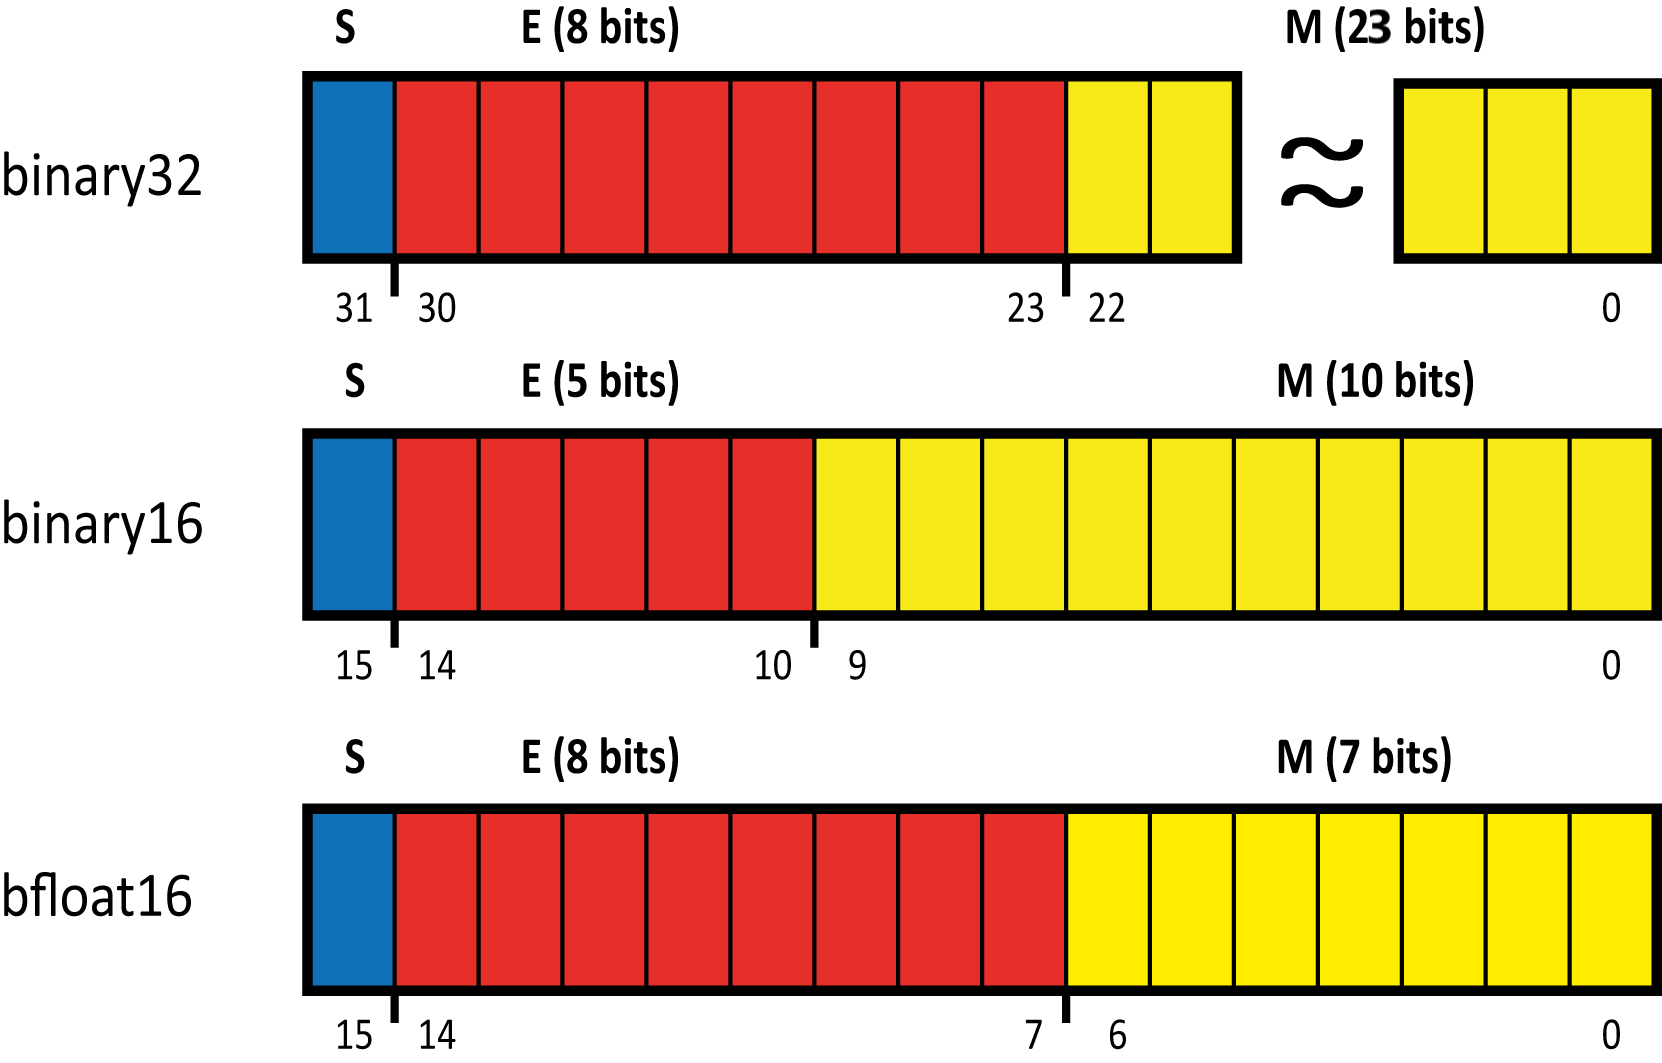
\includegraphics{float.png}	
	\caption{How the bits are assigned in the different standards. \\From top to bottom: binary32, binary16, bfloat16}
\end{figure}

Heap Lab has already developed an open source FPU (\url{https://gitlab.com/davide.zoni/bfloat_fpu_systemverilog}) supporting the most common operations for bfloat16 operands. \\
However, it still misses some other important operations, such as the fused Multiply-Add and the Square Root. We are requested to implement one of these operations, in particular we have chosen to develop the Square Root algorithm.\\

More formally, the goals of our project are:
\begin{itemize}
	\item Add support for Square Root operation
	\item Verify the implementation correctness, comparing the results produced by our design with the ones obtained from the 		C function sqrt
	\item Add support for the INVSQRT operation
\end{itemize}

\clearpage

\section{Goldschmidt’s algorithm} \label{goldschmidt}
The Square Root is quite complicated from a computational point of view; in fact, the most efficient known algorithms require to compute this operation by using an iterative approach, involving a chain of multiplications and other operations. The two most famous algorithms are the Newton-Raphson iterations are Goldschmidt’s algorithm. The latter has been chosen for bfloat16, since it's suitable for an efficient hardware implementation. 
\\
Given a Significand $S$, Goldschmidt's algorithm can be used to compute $\sqrt{S}$. Withonly one small variations, it's also possible to compute $\frac{1}{\sqrt{S}}$.\\
The objective is to find a series of $R_0$, $R_1$, ... , $R_n$ such that the following product tends to 1:
$$B_n = S*R_0^{2}*R_1^{2}* ... * R_{n-1}^{2} \approx 1 $$
Then, we can approximate the Square Root as:
$$ X_{n} = S * R_0*R_1* ... * R_n \approx \sqrt{S} $$
And the Inverse Square Root as:
$$ Y_n =   R_0*R_1* ... * R_n \approx  \frac{1}{\sqrt{S}}$$
\\
Goldschmidt's algorithm initializes its variables as follow:

\begin{itemize}
\item $B_0$ = S
\item $Y_0$ = $R_0$ = $\frac{3-S}{2}$
\item $X_0$ = S * $R_0$
\end{itemize}

Each Goldschmidt's iteration firstly consist of computing:

\begin{enumerate}
\item $B_i$ = $B_{i-1}$ * $R_{i-1}^{2}$
\item $R_i$ = $\frac{3-B_i}{2}$
\end{enumerate}

And secondly it updates the Square Root and the Reciprocal Square Root approximations as follow:
\begin{enumerate}
\item $X_i$ = $X_{i-1}$ * $R_i$
\item $Y_i$ = $Y_{i-1}$ * $R_i$
\end{enumerate}

Iterations stops when R reaches a good approximation of 1 or when $X_i$ reaches M bits of precision; the latter condition can be achieved with a fixed amount of iterations that depends on M (in our case, 8 bits).\\

We wanted to show that the Goldschmidt algorithm is very efficient, as it requires only a very small number of iterations to reach the desired precision. To do so, we quickly implemented the algorithm in Matlab and tracked the values of $B_i$, $R_i$, $Y_i$ and $X_i$ for ten iterations.\\ The code (\ref{fig:Matlab_Algorithm}) is simply the software implementation of the algorithm, and we run it twice; the first time, we put $S$ = 1,5625, which yelds an exact Square Root (\ref{fig:S_15625}).
 The second time, we used $S$ = 1,5, which instead yelds an irrational number as solution (\ref{fig:S_15}).\\
In both cases, the algorithm converges in 5 or 6 iterations. Given that we only use 8 bits for the Mantissa, and not 24 like Matlab, we'll reach the desired precision in even fewer iterations.

\begin{figure}[h]
	\centering
	\captionsetup{justification=centering}
	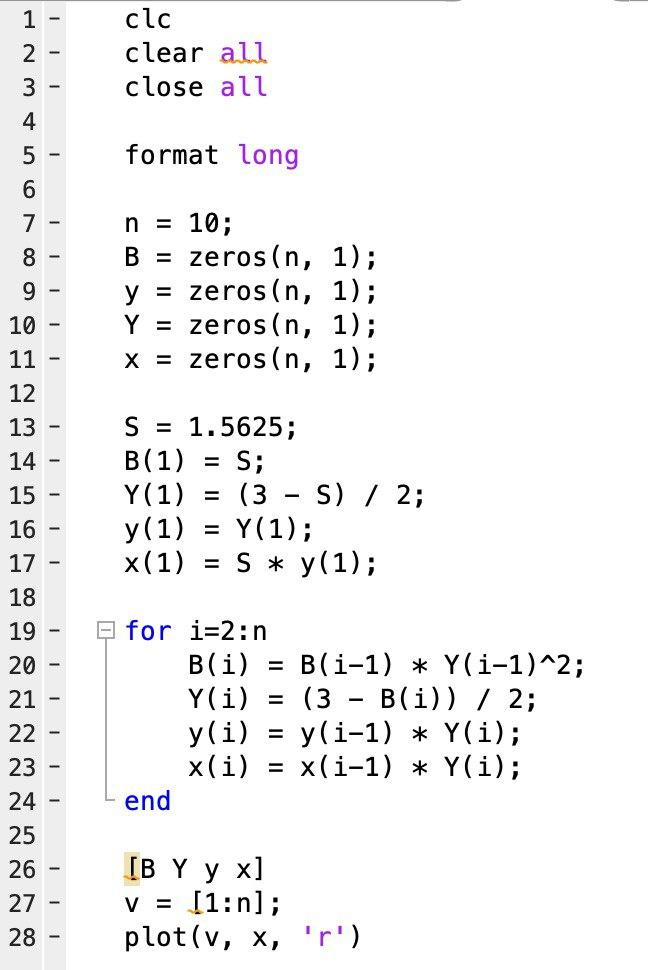
\includegraphics[scale=0.5]{Matlab_Algorithm.jpg}	
	\caption{Goldschmidt's algorithm implemented in Matlab}
	\label {fig:Matlab_Algorithm}
\end{figure}

\begin{figure}[h]
	\centering
	\captionsetup{justification=centering}
	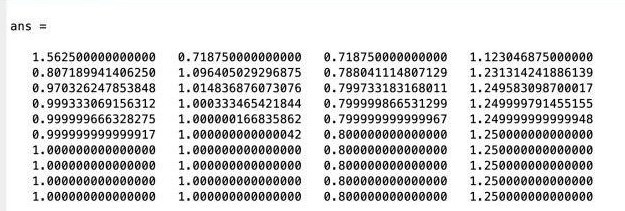
\includegraphics[scale=0.7]{S_15625.jpg}	
	\caption{Results with S = 1,5625\\From left to right, the values of B, R, Y, X}
	\label {fig:S_15625}
\end{figure}


\begin{figure}[h]
	\centering
	\captionsetup{justification=centering}
	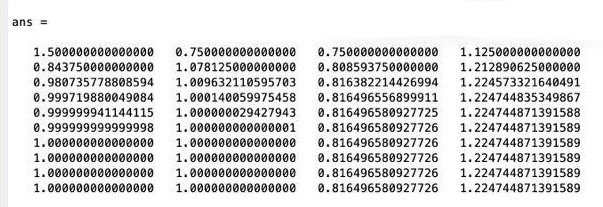
\includegraphics[scale=0.7]{S_15.jpg}	
	\caption{Results with S = 1,5\\From left to right, the values of B, R, Y, X}
	\label {fig:S_15}
\end{figure}

\clearpage


\section{Design and Implementation} \label{design}
For our project we used the Hardware Description Language (HDL) SystemVerilog. SystemVerilog allows to create a device-independent representation of digital logic and is the de-facto standard for digital design and especially for verification (together with VHDL). 
In SystemVerilog, the \emph{modules} are the basic building blocks. SystemVerilog design consists in interconnected modules.
Our implementation is based on two new interconnected modules together with the original FPU, properly modified:

\begin{itemize}
\item \emph{lampFPU\_sqrt.sv} is the top module, called from the external component of the FPU; it mainly computes the exponent of the number we want the Square Root (or Inv Square Root) of, manages some special cases (Square Root of NaN, Square Root of negative number, etc.) and instantiates \emph{lampFPU\_fractSqrt.sv}
\item \emph{lampFPU\_fractSqrt.sv} implements Goldschmidt's algorithm for the Mantissa of a bfloat16 number. 
\item Our source code also uses some functions and constants in order to make the design parametric. We imported the already existing package \emph{lampFPU\_pkg.sv} containing some useful parameters. We then added some other values and functions we needed. We highlight that in doing so we greatly accelerated the integration process of our modules with the rest of the FPU.
\item We modified \emph{lampFPU\_top.sv} in order to properly manage the square root operation, adding the required internal wires, instantiating our new module \emph{lampFPU\_sqrt.sv} and binding the inputs and outputs to it. We assigned the square root to the operation code 10 and to the inverse square root to 11. 
\item The folder Source\_Code also contains other SystemVerilog files already implemented for the bfloat16 FPU. We need these modules because \emph{lampFPU\_top.sv} instantiates them.
\end{itemize}

The Square Root algorithm requires to compute not only the Mantissa, but the exponent too. \emph{lampFPU\_sqrt.sv} and  \emph{lampFPU\_fractSqrt.sv} need to collaborate in order to obtain the correct result. 
\begin{itemize}
\item If the exponent is even, we simply divide it by 2 in the external module \emph{lampFPU\_sqrt.sv}  (so we right shift the exponent).
\item If the exponent is odd, simply right shifting would not produce the right result. In order to compute the correct final value, we make the exponent even by exploiting:
$$F = (-1)^{S}*M*2^{E}  = (-1)^{S}*(M*2)*2^{E-1} $$
We can now divide by 2 the exponent and we inform the internal module that the exponent was odd with the input \emph{is\_exp\_odd\_i}. \\
We then exploit a well-known property of the Square Root:
$$ \sqrt{2*M} = \sqrt{2} * \sqrt{M} $$
So, we actually pass M (and not $2 * M$) to the internal module, but we multiply the result computed by Goldschmidt's algorithm by $\sqrt{2}$ before returning it.\\
The same mathematical properties are applied when we want to compute the inverse square root, but in this case, we exploit:
$$ \sqrt{\frac{1}{2*M}} = \frac{1}{\sqrt{2} * \sqrt{M}} $$
\end{itemize} 

\subsection{lampFPU\_fractSqrt.sv}
We firstly describe the lampFPU\_fractSqrt.sv module. \\
In general, \emph{lampFPU\_fractSqrt.sv} takes as input an 8-bits Mantissa M between 1.0 (8b'100000000) and 1.9921875 (8b'11111111) and some flags indicating when to start the computation (\emph{doSqrt\_i}), whether to compute the square root or the inverse square root ({invSqrt\_i}), if we are in a special case (emph{special\_case\_i}).\\
The module signals it finished its work with the output valid\_o, and returns 16 bits representing $\sqrt{M}$ or $\frac{1}{\sqrt{M}}$. The Mantissa length is greater than expected by the bfloat16 standard, but we'll use this enhanced precision in order to properly round the result when needed.\\\\
The sequential logic of \emph{lampFPU\_fractSqrt.sv} implements a synchronous reset of the module, setting to zero all the internal wires if the input \emph{rst} is 1. Otherwise, it saves the values computed by the combinational logic into internal registers.\\\\
The combinational logic of \emph{lampFPU\_fractSqrt.sv} implements a Finite State Machine with four different states:
\begin{enumerate}
\item Every times it starts, we compute the various values required by the algorithm, but we don't save them until we're in the right state.
\item In the IDLE state, we initialize our internal variables as described in Section \ref{goldschmidt}, only if the external input \emph{doSqrt\_i} signals to start the computation and we're not in one of the special cases (Square Root of NaN, Square Root of Zero...). To note, we declare the number 3 as 9'b110000000; since our Significant occupies 8 bits and is between 1.0 and 1.9921875, in order to represent the number 3 we need to add an additional bit. 
\item SQRT\_B is the output state; if $R_i$ is 1, we stop the computation, return the result (either the square root or the inverse square root) and signal the end by setting \emph{valid\_next} as 1. If the exponent of the bfloat16 we want the square root of is odd, we first multiply $X_i$ by $\sqrt{2}$ and $Y_i$ by $\frac{1}{\sqrt{2}}$. Goldschmidt's algorithm doesn't yeld a precise LSB, but we return x\_tmp or y\_tmp, which have more precision than our final result. We delegate the rounding to \emph{lampFPU\_top.sv}. \\
On the other hand, if the estimation of the square root is not good enough, we perform another iteration of the algorithm, by updating \emph{b\_next} and moving to the next state.
\item In the SQRT\_R state, we update $R_i$ as requested by the algorithm.
\item In the SQRT\_XY state, we update $X_i$ and $Y_i$ as requested by the algorithm and move back to SQRT\_B.
\end{enumerate}

\subsection{lampFPU\_sqrt.sv}
We now describe the lampFPU\_sqrt.sv module.\\
In general, \emph{lampFPU\_sqrt.sv} module instantiates \emph{lampFPU\_fractSqrt.sv}, computes the final exponent and manages some special cases. \\ 
The square root is a particular operation, since it can't produce neither an overflow nor an underflow. They occur when positive numbers exceed the maximum value or negative numbers exceed the maximum negative value that can be represented. For the square root, we have that:
\begin{itemize}
\item If $X > 1$, then $X > \sqrt{X} > 1$ 
\item If $0 < X < 1$, then $0 < X < \sqrt{X} < 1$
\item If $X < 0$, then $\sqrt{X}$ is NaN
\end{itemize}
This means that if X is a number that can be represented in bfloat16, its square root can always be represented in bfloat16. For this reason, \emph{lampFPU\_sqrt.sv} doesn't need to manage overflow or underflow cases.\\ \\
% add why don't need normalization
%add module interface%
lampFPU\_sqrt.sv takes as inputs the operand we want the square root of, already divided in signum, exponent and mantissa. Some flags states whether the input is NaN, Zero or Infinity. The module returns the square root of the inputs, still split in signum, exponent and mantissa, as well as a flag signaling if the result needs to be rounded.\\\\
The sequential logic of  \emph{lampFPU\_sqrt.sv} resets to zero the module's internal wires and the outputs when the input \emph{rst} is 1. Otherwise, it saves some of the inputs into internal registers and updates the outputs.\\\\
The combinational logic of \emph{lampFPU\_sqrt.sv} firstly checks if we're trying to compute the Square Root or Inverse Square Root of a special case, using the function \emph{FUNC\_calcInfNanZeroResSqrt}. In this case, the output doesn't need to be rounded. We have the following:
\begin{itemize}
\item $\sqrt{+0}$ = $+0$ 
\item $\sqrt{-0}$ = $-0$
\item $\sqrt{NaN}$ = NaN
\item $\sqrt{+ \infty}$  =  $+\infty$
\item $\sqrt{- \infty}$ =  NaN
\item $\sqrt{- X}$ = NaN  (X is any generic number) 
\item $\frac{1}{\sqrt{+0}}$ = NaN
\item $\frac{1}{\sqrt{-0}}$ = NaN
\item $\frac{1}{\sqrt{NaN}}$ = NaN (Inf???)
\item $\frac{1}{\sqrt{+\infty}}$ = $+0$
\item $\frac{1}{\sqrt{-\infty}}$ = NaN
\item $\frac{1}{\sqrt{-X}}$ = NaN  (X is any generic number) 
\end{itemize}

If we are not in a special case, we compute the exponent and wait until the internal module computes the square root or inverse square root of the Mantissa (we uses  \emph{srm\_valid} for it) and then we return the final value as outputs. To note, the signal \emph{f\_res\_o} has a dimension of 12 bits, that are:
\begin{itemize}
\item The MSB is the overflow bit; as discussed before, this bit will always be zero
\item Bits from 10\textsuperscript{th} to 3\textsuperscript{th} represent the "real" mantissa, as expected by bfloat16 standard.
\item The Ground bit is the bit immediately on the left of the Mantissa LSB, so it's the 2\textsuperscript{th} bit of \emph{f\_res\_o}.
\item The Round bit is on the left of the Ground bit, so it's the 1\textsuperscript{rd} bit of \emph{f\_res\_o}.
\item The Sticky bit is computed as the logical or of three bits of \emph{f\_initial} (which has 16 bits of precision), and is the LSB of \emph{f\_res\_o} . 
\end{itemize}
These additional bits are used for rounding, which is delegated to the top module; we inform the top module with the signal \emph{isToRound}. The rounding is performed using the function \emph{FUNC\_rndToNearestEven} which implements the following rules:
\begin{itemize}
\item If GRS = 0XX, then round down
\item If GRS = 100, then round up if mantissa LSB is 1, otherwise round down
\item Any other case, round up
\end{itemize} 

\clearpage


\section{Experimental Results} \label{results}
\subsection{Test Setup}
In order to properly validate our implementation, we tested our design using a test-bench; this test-bench can generate random numbers, compute the results of our implementation and then compare them with the results of the C function \emph{sqrtf} (that can be found in \emph{math.h}).  \\
All the other functions and operations already developed for the FPU were tested this way, so we extended two existing files:
\begin{itemize}
\item dpi\_lampFPU.c is a C file; we added the functions \emph{DPI\_sqrt} and \emph{DPI\_invSqrt}. Given a value X, They return the value of $\sqrt{X}$ and $\frac{1}{\sqrt{X}}$, as unsigned integer representing a number in binary32.
\item tb\_lampFPU.sv is a SystemVerilog file; it instantiates the FPU, imports the C functions and compares their results with the ones produced by the top module. 
\end{itemize}

In order to test our implementation, we added two different tasks:
\begin{itemize}
\item \emph{TASK\_doSqrt\_op} takes as input the number X we want the square root of, calls the right C function defined in dpi\_lampFPU.c depending on the opcode, and saves the result. Then, the task rounds this result and compute $\sqrt{X}$ or $\frac{1}{\sqrt{X}}$ using our implementation. Then, the two results are compared. If they're the same, the test is passed, otherwise it fails. 
\item \emph{TASK\_testSqrt} creates a loop with 5000 iterations; in each one, it randomly generates values for the sign, the exponent and the mantissa, and calls \emph{TASK\_doSqrt\_op}. It also manages all the special cases, explicitly creating a test for each of them. 
\end{itemize}

\subsection{Results}
We ran our test-bench using the Vivado software, performing a behavioural, post-synthesis and post-implementation simulation.\\
The results completely validate our implementation; out of 5000 tests performed, we're able to correctly compute the square root of all of them, obtaining zero rejections. \\
For the inverse square root, instead, we have a very small set of tests rejected (21 out of 5000, the 0,42\%); in all these cases, our implementation returns the right exponent and sign, but has a mantissa one bit greater than expected. The issue probably lies in the rounding function, since the mantissa computed by our implementation is very close to the right value.  

\subsection{Algorithm Simulation}
In this section we show the efficiency of the algorithm for one randomly selected value. In order to keep the description as simple as possible, we will focus only on some signals and their values.\\ 
In the following pictures, the colour red is reserved to the clock and reset signals, the light blue to the module lampFPU\_sqrt.sv and the green to the module lampFPU\_fractSqrt.sv \\
\begin{figure}[h]
	\centering
	\captionsetup{justification=centering}
	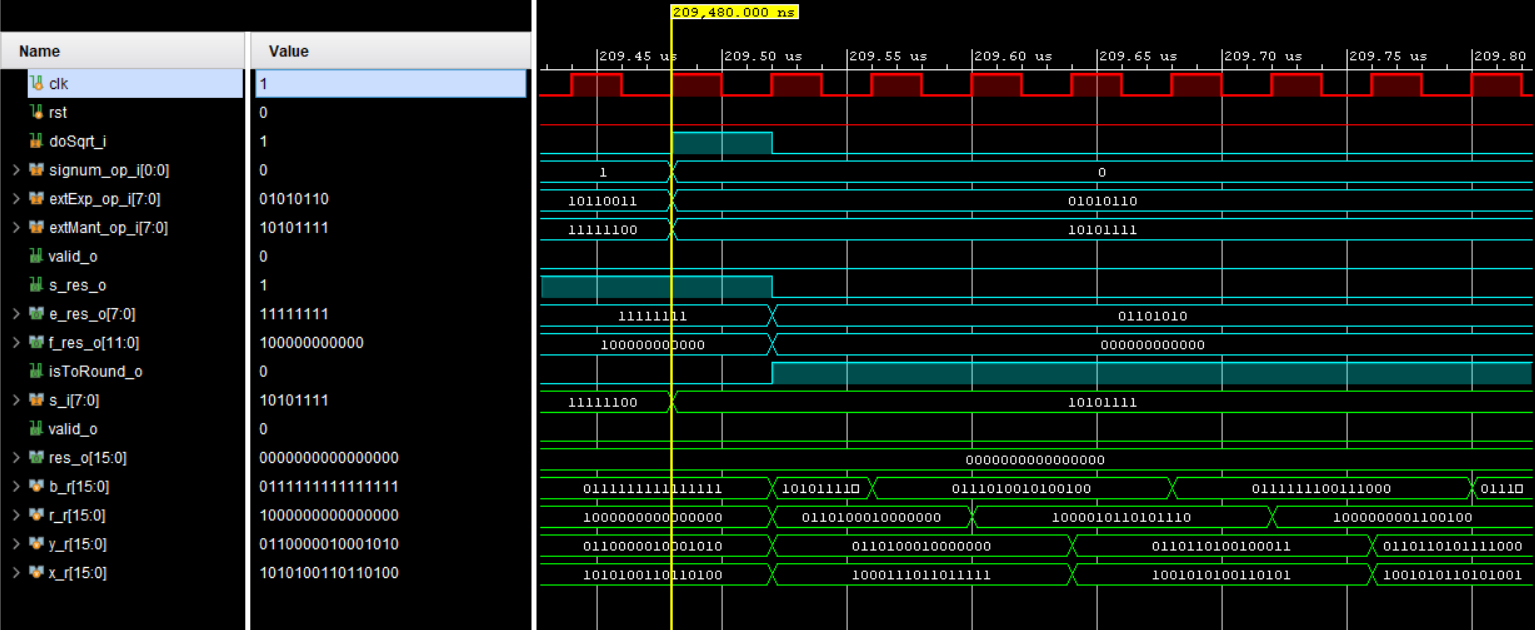
\includegraphics[width=\linewidth]{Simulation0.png}	
	\caption{First part of the simulation}
\end{figure}

\begin{itemize}
\item The test start at time 209.48 $\mu$s, when the signal doSqrt\_i is set to 1. We can see from the blue signals just under doSqrt\_i that the input number is positive, has exponent 01010110 and mantissa 10101111, so is the decimal number $6.217249*10^{-13}$; the mantissa, considered without the exponent, is the decimal number 1.3671875. We need a clock cycle before this information is propagated to the inner module, lampFPU\_fractSqrt.sv (green signals), which still has some values left from the previous test. We remember that for each internal signal shown in this simulation (for example b\_r) there is another one (b\_r\_next), not visualized for clarity.
\item In the next clock cycle (209.52 $\mu$s), lampFPU\_sqrt.sv recognizes we're not in a special case, so it computes the final exponent and sets \emph{isToRound\_o} to 1. Now, this module will wait until the inner one finishes its task.\\
In lampFPU\_fractSqrt.sv, all the internal registers are initialized. We refer to Section \ref{goldschmidt} for a complete description of the algorithm; since it's the first iteration, $B_0$ is set to the extended mantissa input and $Y_0$ is equal to $R_0$. 
\item In the next clock cycles we can see the evolution of the algorithm; depending on the current state, we update b\_r, r\_r, or y\_r and x\_r. To note, r\_r from the first to the second cycle becomes grater than 1, but then it keeps decreasing.
\item After only 10 clock cycles, r\_r becomes exactly 1; we need two more clock cycles in order to propagate the computed result. We can see that: 
$$x_r = 1001010110101001$$However, the input exponent is odd ($01010110$, or $-41$), so we need to multiply
$x_r * \sqrt{2}$. At time $209.92 \mu$s the inner module sets \emph{valid\_o} to 1 and gives us the final result, that is $1101001110100110$, or $1.6535034$ The Windows calculator instead computes $1.65359457$. 
\item This result is passed to the outer module, that returns it to lampFPU\_top.sv, putting the overflow bit to 0, computing the sticky bit and setting \emph{valid\_o} to 1. The 12 bits now are:
$$f\_res\_o = 011010011101$$ 
\item The top module now rounds the results (not shown in the diagram); using the rounding rules described in Section \ref{design}, we obtain the final value of the mantissa:
$$ M = (1)1010100 = 1.65625$$
This value is a bit greater than the real one but we have to remember that we only have 8 bits of precision; indeed, decreasing by 1 the alternative value would be:
 $$ M' = (1)1010011 =1.6484375$$
The difference between M' and the real value is greater than the one obtained with M.
\item The test finishes and prints the results (fig. \ref{simRes}). We can see that it passes the test.
\end{itemize}
\begin{figure}[h]
	\centering
	\captionsetup{justification=centering}
	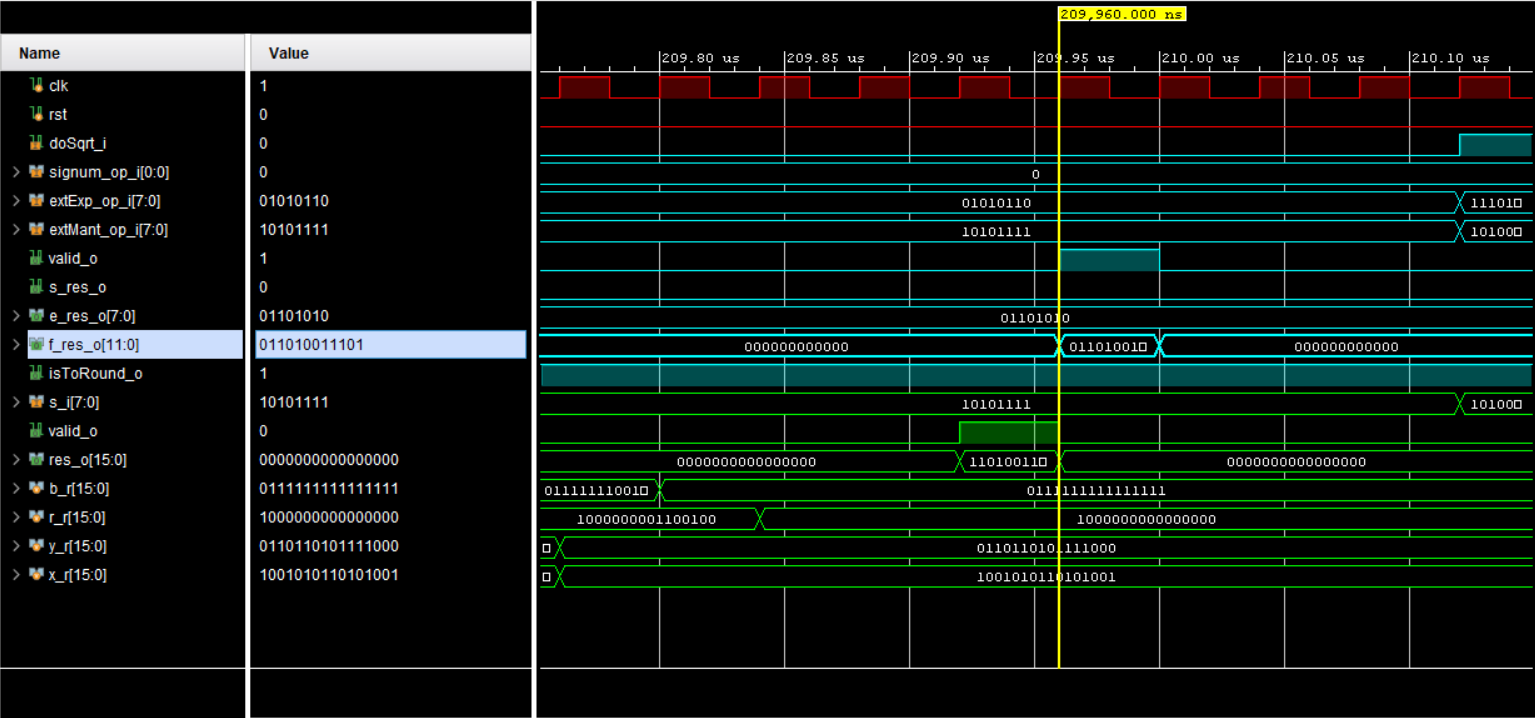
\includegraphics[width=\linewidth]{Simulation1.png}	
	\caption{Second part of the simulation}
\end{figure}
\begin{figure}[h]
	\centering
	\captionsetup{justification=centering}
	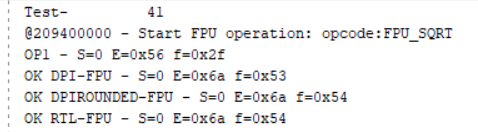
\includegraphics[width=\linewidth]{SimulationResult.png}	
	\caption{Final results of the simulation}
	\label{simRes}
\end{figure}





\clearpage

\section{Conclusions} \label{conclusions}
\clearpage


\end{document}
